%%%%%%%%%%%%%%%% Springer %%%%%%%%%%%%%%%%%%%%%%%%%%%%%%%%%%
% RECOMMENDED %%%%%%%%%%%%%%%%%%%%%%%%%%%%%%%%%%%%%%%%%%%%%%%%%%%
\documentclass[graybox]{svmult}
% choose options for [] as required from the list
% in the Reference Guide
\usepackage{type1cm}        % activate if the above 3 fonts are
                            % not available on your system
%
\usepackage{makeidx}         % allows index generation
%\usepackage{graphicx}        % standard LaTeX graphics tool
                             % when including Fig.~files
\usepackage{multicol}        % used for the two-column index
\usepackage[bottom]{footmisc}% places footnotes at page bottom
\usepackage{newtxtext}       % 
\usepackage{newtxmath}       % selects Times Roman as basic font
% see the list of further useful packages
% in the Reference Guide
%\makeindex             % used for the subject index
                       % please use the style svind.ist with
                       % your makeindex program
%%%%%%%%%%%%%%%%%%%%%%%%%%%%%%%%%%%%%%%%%%%%%%%%%%%%%%%%%%%%%%%%%%%%%%%%%%%%%%%%%%%%%%%%%
% \usepackage{amsmath}
% \usepackage{ascmac}
\usepackage[dvipdfmx]{graphicx}  % for EPS and PDF 
% \usepackage{url}
\usepackage{fancyvrb}
% \usepackage{makeidx}
% \usepackage{float}
% \usepackage[dvipdfmx]{color}
% \usepackage{ulem}
% \usepackage[switch*,pagewise]{lineno}
% \usepackage[dvipdfm,bookmarkstype=toc,urlcolor=black,%
%     linkcolor=black,citecolor=black,bookmarks=false]{hyperref}
% \usepackage{fancyhdr}

\usepackage{listings}
\lstset{%
 language={C},
% basicstyle={\scriptsize},%
% identifierstyle={\scriptsize},%
 basicstyle={\small},%
 identifierstyle={\small},%
% commentstyle={\small\itshape},%
%commentstyle={\scriptsize},%
commentstyle={\small},%
 keywordstyle={\small\bfseries},%
 ndkeywordstyle={\small},%
stringstyle={\small\ttfamily},
 frame={tb},
 breaklines=true,
 columns=[l]{fullflexible},%
 numbers=left,%
 xrightmargin=1zw,%
 xleftmargin=1.5zw,%
 numberstyle={\small},%
 stepnumber=1,
 numbersep=1zw,%
% lineskip=-0.1ex%
}

\def\|{\verb|}

%\newenvironment{myfigure}{\begin{figure}[ht]\begin{center}}{\end{center}\end{figure}}

\def\Directive#1{{\tt #1}\index{#1@{\tt #1}}\index{Directive!#1@{\tt #1}}}

%\def\Syntax#1{\index{{\tt #1}}\index{Syntax!{\tt #1}}}
\def\Syntax#1{\index{Syntax!#1@{\tt #1}}}

\def\Term#1{{#1}\index{#1}}

%\def\Example#1{\index{#1}\index{Example!{\tt #1}}}
\def\Example#1{\index{Example!#1@{\tt #1}}}

\def\Intrinsic#1{\index{#1@{\tt #1}}\index{Intrinsic and Library Procedures!#1@{\tt #1}}}

\DefineVerbatimEnvironment{Fexample}{Verbatim}{numbers=left,numbersep=3pt,stepnumber=5,%
frame=single,label=\Fort}
\DefineVerbatimEnvironment{FexampleR}{Verbatim}{numbers=right,numbersep=3pt,stepnumber=5,%
frame=single,label=\Fort}

\DefineVerbatimEnvironment{Cexample}{Verbatim}{numbers=left,numbersep=3pt,stepnumber=5,%
frame=single,label=\C}
\DefineVerbatimEnvironment{CexampleR}{Verbatim}{numbers=right,numbersep=3pt,stepnumber=5,%
frame=single,label=\C}

\DefineVerbatimEnvironment{XFexample}{Verbatim}{numbers=left,numbersep=3pt,stepnumber=5,%
frame=single,label=\XMPF}
\DefineVerbatimEnvironment{XFexampleR}{Verbatim}{numbers=right,numbersep=3pt,stepnumber=5,%
frame=single,label=\XMPF}

\DefineVerbatimEnvironment{XCexample}{Verbatim}{numbers=left,numbersep=3pt,stepnumber=5,%
frame=single,label=\XMPC}
\DefineVerbatimEnvironment{XCexampleR}{Verbatim}{numbers=right,numbersep=3pt,stepnumber=5,%
frame=single,label=\XMPC}

\DefineVerbatimEnvironment{MPICexample}{Verbatim}{numbers=right,numbersep=3pt,stepnumber=5,%
frame=single,label=MPI C}
\DefineVerbatimEnvironment{MPIFexample}{Verbatim}{numbers=right,numbersep=3pt,stepnumber=5,%
frame=single,label=MPI Fortran}


\setcounter{secnumdepth}{4}
\setcounter{tocdepth}{3}
\setcounter{totalnumber}{6}
\usepackage{fancyhdr}

\let\olditemize\itemize
\renewcommand{\itemize}{
   \olditemize
   \setlength{\itemsep}{8pt}
   \setlength{\parskip}{0pt}
   \setlength{\parsep}{0pt}
}

% \parindent = 0pt
% \hoffset=0cm
% \oddsidemargin=0cm
% \evensidemargin=0cm
% \textwidth=16cm
% \topmargin=-1cm
% \voffset=0cm
% \textheight=24cm

\def\progenv{\baselineskip=10pt\tt\progspecial{`}\parindent=0.3cm}
\def\shellenv{\baselineskip=10pt\tt\progspecial{`}\parindent=0.3cm\nolineno}

\renewcommand{\topfraction}{.99}
\renewcommand{\bottomfraction}{.99}

\def\openb{{\it [}}
\def\closeb{{\it ]}}
\def\XMP{XcalableMP}
\def\XACC{XcalableACC}
\def\OACC{OpenACC}
\def\OMP{OpenMP}
\def\XMPF{XcalableMP Fortran}
\def\XMPC{XcalableMP C}
\def\XACCF{XcalableACC Fortran}
\def\XACCC{XcalableACC C}
\def\Syntax#1{\index{Syntax!#1@{\tt #1}}}
\def\Example#1{\index{Example!#1@{\tt #1}}}
%
\def\phrule{\vspace{0.2cm}\hrule\vspace{0.05cm}\hrule}
\def\qhrule{\vspace{0.2cm}\hrule}
\def\dhrule{\hrule\vspace{0.05cm}\hrule}
\def\bsquare{\rule[-2pt]{5pt}{10pt}}
%
\newenvironment{mytable}[3]{\begin{table}[ht]\caption{#1}\label{#2}\vspace*{-0.3cm}\begin{center}\begin{tabular}{#3}}{\end{tabular}\end{center}\end{table}}
\newenvironment{myfigure}{\begin{figure}[ht]\begin{center}}{\end{center}\end{figure}}
%
\DefineVerbatimEnvironment{XACCFexampleL}{Verbatim}{numbers=left,numbersep=3pt,stepnumber=5,frame=single,label=\XACCF}
\DefineVerbatimEnvironment{XACCCexampleR}{Verbatim}{numbers=right,numbersep=3pt,stepnumber=5,frame=single,label=\XACCC}
\DefineVerbatimEnvironment{XACCCexampleL}{Verbatim}{numbers=left,numbersep=3pt,stepnumber=5,frame=single,label=\XACCC}

%%%%%%%%%%%%%%%%%%%%%%%%%%%%%%%%%%%%%%%%%%%%%%%%%%%%%%%%%%%%%%%%%%%%%%%%%%%%%%%%%%%%%%%%%

% my definitions
\newcommand{\requirement}{{\bf Requirement to the implementation.} }
\newcommand{\fig}[1]{Figure~\ref{fig:#1}}
\newcommand{\tab}[1]{Table~\ref{tab:#1}}
\newcommand{\Sec}[1]{Section~\ref{sec:#1}}


%%%%%%%%%%%%%%%%%%%%%%%%%%%%%%%%%%%%%%%%%%%%%%%%%%%%%%%%%%%%%%%%%%%%%%%%%%%%%%%%%%%%%%%%%


\begin{document}



\title*{Coarrays in the Context of XcalableMP}
% Use \titlerunning{Short Title} for an abbreviated version of
% your contribution title if the original one is too long

\author{H.\ Iwashita and M.\ Nakao}
% Use \authorrunning{Short Title} for an abbreviated version of
% your contribution title if the original one is too long

\institute{
Hidetoshi Iwashita 
\at Fujitsu Limited, 140 Miyamoto, Numazu-shi, Shizuoka 410-0396, Japan,
\email{iwashita.hideto@fujitsu.com}
\and
Masahiro Nakao \at RIKEN Center for Computational Science,
7-1-26 Minatojima-minami-machi, Chuo-ku, Kobe, Hyogo 650-0047, Japan,
\email{masahiro.nakao@riken.jp}
}

%
% Use the package "url.sty" to avoid
% problems with special characters
% used in your e-mail or web address
%
\maketitle

\abstract{
Coarray features has been implemented into the Omni XcalableMP compiler
with a source-to-source translator and layered runtime libraries.
%
Three memory allocation methods for coarrays were implemented for
communication libraries GASNet, MPI-3 and Fujitsu's native interface.
%
For the coarray PUT/GET communication, algorithms using DMA (zero-copy) 
and buffering were introduced. The important techniques for achieving 
high performance were the non-blocking PUT communication implemented 
in the runtime library and the optimization for the GET communication 
in the translator.
%
Using the ping-pong benchmark and the modified version, the fundamental
performance was evaluated and analyzed.
The MPI version of the Himeno benchmark is ported to coarray version
and modified for fully using the non-blocking PUT. 
As the result of the evaluation, non-blocking coarray version clearly 
outperformed the original and non-blocking MPI versions.
}

%\tableofcontents
%\clearpage

%
% Sections
%
\section{Introduction}\label{chap:intro}

\pagenumbering{arabic}
\setcounter{page}{1}

XcalableMP (XMP)~\cite{xmp} has complementary programming models of
global-view and local-view. The former is a directive-base language 
extension to the base language Fortran and C, and the latter adopts 
the coarray features defined in Fortran 2008~\cite{coarray} and 
a part of the ones in Fortran 2018~\cite{coarray18}. 
%
The purpose of the coarray features as the local-view part of XMP is 
1) writing the application programs that is difficult for the global-view programming
and 2) writing such important parts of the program that is critical for the performance
with easier programming model than the MPI message passing.
Therefore, the coarray features in XMP must be naturally merged into the 
global-view XMP language and must perform with high performance comparable to MPI.

The Omni XMP compiler is an open-source implementation developed at RIKEN 
and the University of Tsukuba~\cite{omni}. 
Its kernel is a source-to-source compiler that converts an XMP program 
into a Fortran program by calling a runtime library.
%
The coarray translator has been implemented into the Omni XMP compiler.
Since the images is mapped one-to-one to XMP nodes, 
each image was implemented as a process, and 
the definition and reference to coarrays were implemented as the 
inter-node one-sided communications.

This chapter describes the techniques in the coarray compiler and 
the runtime library with some evaluation compared with the MPI message passing.
In the rest of this chapter, 
Section 2 introduces the requirements from the coarray features,
Section 3 describes the implementation to solve the requirements, and
Section 4 evaluates the performance and the productivity of coarray programs.
After related work is shown in Section 5, Section 6 concludes this chapter.


 

\section{Requirements from Language Specifications}\label{sec:spec}

XMP Fortran language specification~\cite{xmp} supports a major part of 
coarray features defined in Fortran~2008 standard~\cite{coarray}, 
and intrinsic procedures {\tt CO\_SUM}, {\tt CO\_MAX}, {\tt CO\_MIN} and 
{\tt CO\_BROADCAST} defined in Fortran~2018 standard~\cite{coarray18} were supported.
And also XMP C language specification extended to support coarray features.

This section introduces the coarray features and what is required
to the compiler in order to implement the coarray features.


%-----------------------------------------------------------------------------
\subsection{Images Mapped to XMP Nodes}\label{sec:spec-image}
%-----------------------------------------------------------------------------

In the Fortran standard, an {\bf image} is defined as a instance of a program. 
Each image executes the same program and has its own data individually.
Each image has a different image index $k$.
While the Fortran standard itself does not specify where each image is executed, 
XMP specifies that images are mapped to executing nodes on a one-to-one basis.
Therefore, image $k$ is always executed on executing node $k$, where $1 \leq k \leq n$ and 
$n$ is the number of images and also the number of the executing nodes. 
Since each MPI rank number of {\tt MPI\_COMM\_WORLD} (0-origin) is 
always mapped to an XMP node number in order, image $k$ is corresponding to 
rank $(k - 1)$.

Note that the executing nodes can be a subset of the entire (initial) node set. 
For example, two distinct node sets can execute two coarray subprograms concurrently.
The first executing images at the start of the program is the entire images.
Coarray features are compatible to the ones of the Fortran standard unless 
the {\tt TASK} and {\tt END TASK} directives are used.
If the execution encounters a {\tt TASK} directive specified with a subset of nodes, 
the corresponding subset of the images will be the executing images for the task region. 
The current number of images and my image number, which are given by inquire functions
{\tt num\_images} and {\tt this\_image}, also match with the executing images, and
the {\tt SYNC\_IMAGES} statement synchronizes among the executing images.
When the execution encounters the {\tt END TASK} directive corresponding to the
{\tt TASK} directive, the set of executing image is reinstated.

%   Coarray features can be used inside the TASK directive blocks. As default,
%   each coarray image is mapped one-to-one to a node of the current executing 
%   task. I.e., num_images() returns the number of nodes of the current executing 
%   task and this_image() returns each image index in the task.
%      There are two directives to change the default rule above. A COARRAY 
%   directive corresponding to a coarray declaration changes the image index set 
%   of the specified coarray with the one of the specified nodes. An IMAGE 
%   directive corresponding to one of a SYNC ALL statement, a SYNC IMAGES 
%   statement, a call statement calling CO_SUM, CO_MAX, CO_MIN or CO_BROADCAST 
%   changes the current image index set with the one of the specified nodes.
%   See the language spacifications [3].

\requirement
The runtime library should manage the executing image set and the current image index 
in stack in order to reinstate them at the exit point of the task.


%-----------------------------------------------------------------------------
\subsection{Allocation of Coarrays}\label{sec:spec-coarray}
%-----------------------------------------------------------------------------

A {\bf coarray} or a coarray variable is a variable that can be referred from the other images. 
A coarray with the {\tt ALLOCATABLE} attribute is called an {\bf allocatable coarray}, 
otherwise called a non-allocatable coarray. A non-allocatable coarray may not be a pointer 
and must have an explicit shape and the {\tt SAVE} attribute. In order to help 
intuitive understanding, we call a non-allocatable coarray as a {\bf static coarray}. 
The lifetime of a static coarray is throughout execution of the program on all images even if
the coarray is declared in a procedure called with a subset of images.

On the other hand, an allocatable coarray is allocated with the {\tt ALLOCATE} statement and 
freed either explicitly with the {\tt DEALLOCATE} statement or implicitly at the end of the 
scope in which the {\tt ALLOCATE} statement is executed ({\bf automatic deallocation}).

Static coarrays can be declared as scalar or array variables as follows:
\begin{verbatim}
      real(8), save :: a(100,100)[*]
      type(user_defined_type), save :: s[2,2,*]
\end{verbatim}

The square bracket notation in the declaration distinguishes coarray variables from 
the others (non-coarrays). It declares the virtual shape of the images and the last 
dimension must be deferred (as `{\tt *}').

Allocatable coarrays can be declared as follows:
\begin{verbatim}
      real(8), allocatable :: b(:,:)[:]
      type(user_defined_type), allocatable :: t[:,:,:]
\end{verbatim}


A notable constraint is that at any synchronization point in program execution, 
coarrays must have the same dimensions (sizes of all axes) between all images
({\bf symmetric memory allocation}). 
Therefore, an static coarray must have the same shape between all images during 
the program execution, and an allocatable coarray must be allocated and deallocated 
collectively at the same time with the same dimensions between the executing images.
Thanks to the syn-metric memory allocation rule, all executing images can have
the same symmetrical memory layout, which makes it possible to calculate the address 
of the remote coarray with no prior inter-image communication.

\requirement
Static coarrays must be allocated and made accessible remotely
before the execution of the user program, and 
made inaccessible remotely and be freed after the execution of the user program.
In contrast, 
allocatable coarrays must be allocated and made accessible remotely
when the {\tt ALLOCATE} statement is encountered, and 
made inaccessible remotely and be freed when the {\tt DEALLOCATE} statement or 
the exit point of the scope that the corresponding {\tt ALLOCATE} statement is encountered 
is encountered.


%-----------------------------------------------------------------------------
\subsection{Communication}\label{sec:spec-comm}
%-----------------------------------------------------------------------------

Coarray features in XMP include three types of communications between images, i.e.,
reference and definition to remote coarrays,
collective communications (intrinsic subroutines {\tt CO\_SUM}, {\tt CO\_MAX}, 
{\tt CO\_MIN} and {\tt CO\_BROADCAST}), and
atomic operations ({\tt ATOMIC\_DEFINE} and {\tt ATOMIC\_REF}).
%
Collective communications and atomic operations are similar to the ones 
in MPI library.
Communication for reference and definition to remote coarrays are 
characteristic for coarray features.


%- PUT communication
PUT communication is caused by an assignment statement with a {\bf coindexed variable} 
as the left-hand side expression, e.g.,
\begin{verbatim}
      a(i,j)[k] = alpha * b(i,j) + c(i,j)
\end{verbatim}
This statement is to cause the PUT communication to the array element {\tt a(i,j)}
on image {\tt k} with the value of the left-hand side.
%
Using Fortran array assignment statement, array-to-array PUT communication 
can be written easily. E.g., the following statement causes 
{\tt M}$\times${\tt N}-element PUT communication.
\begin{verbatim}
      a(1:M,1:N)[k] = alpha * b(1:M,1:N) + c(1:M,1:N)
\end{verbatim}

%- GET communication
GET communication is caused by referencing the {\bf coindexed object}, 
which is represented by a coarray variable with cosubscripts enclosed by square brackets, 
e.g., {\tt s[1,2]} and {\tt a(i,j)[k]}, where {\tt s} and {\tt a} are scalar and 
two-dimensional array coarrays, respectively.
%
A coindexed object can appear almost in any expressions including array expressions.

\requirement
To implement definition/reference to coindexed variable/object,
PUT/GET one-sided communication is suitable to be used.
%
To avoid costly processing such as remote procedure call, 
RDMA (Remote Direct Memory Access)-based implementation is desirable.
%
On PUT/GET communication for large data, redundant multiple memory copies 
should carefully be avoided for all software layers, 
the communication library, the runtime, the Fortran library, and the object.

% A reference of coindexed object is basically converted to a runtime library call
% to get the result of GET communication. 
% Note that the result can be a large array.
% For example, in in array assignment statement:
% \begin{verbatim}
%       c(1:M,1:N) = a(1:M,1:N)[k] + b(1:M,1:N)
% \end{verbatim}
% coindexed object $a(1:M,1:N)[k]$ should be converted to a function that
% returns an array value shaped $[M, N]$.


%-----------------------------------------------------------------------------
\subsection{Synchronization}\label{sec:spec-sync}
%-----------------------------------------------------------------------------

%-- between images
The access order of coarrays between images is explicitly controlled by the 
programmer using the {\bf image control statement}, 
such as {\tt SYNC ALL} and {\tt SYNC IMAGES} statements. 
It allows the compiler system to make PUT/GET communication asynchronous.
The sequence of execution between the image control statements is called 
as a {\bf segment}.
An asynchronous communication must be completed by the end of the segment.

%-- inside image
While, inside each image, the compiler must maintain data dependency 
as before even if it contains coarray communications.
It suppress the {\bf non-blocking communication},
which postpones waiting for communication completion.
In order to keep data dependency among the definitions and references to the same 
coarray in the same segment, the non-blocking communication should be restricted.
The example bellow in which the same remote coarray is accessed some times 
inside the same segment.
\begin{quote}
\begin{verbatim}
 1      if (this_image()==1) then
 2          a[2]=
 3          =a[2]
 4          a[2]=
 5          a[2]=
 6      endif
\end{verbatim}
\end{quote}
Between lines 2 and 3, the completion wait for PUT communication is necessary
to avoid referencing data that is not defined completely.
Similarly, between lines 3 and 4, the completion wait for GET communication is 
necessary to avoid referencing data that is getting updated.
However, between lines 4 and 5, the completion wait is not necessary.
The issue of race condition on image 2 cannot be avoid by the completion wait
on image 1 in general and avoiding it is the matter of the programmer.

\requirement
%To reduce the latency overhead, non-blocking one-sided communication is effective.
%The compiler should generate non-blocking GET communication as long as possible.
Unless the same remote data is accessed from the same segment, 
completion of non-blocking completion is can be delayed until the end of the segment.
%However, the possibility to meet the condition above should 
%be took account. 
Because the data received by the GET communication is usually referenced soon, 
non-blocking GET communication is hard to be used. So if GET communication is
always on blocking, only the flow dependency (between lines 2 and 3) should be care of.


%-----------------------------------------------------------------------------
\subsection{Subarrays and Data Contiguity}\label{sec:spec-contig}
%-----------------------------------------------------------------------------

Except dummy argument, an array is fully {\bf contiguous} across the dimensions.
A subarray of the array can be fully or partially contiguous or non-contiguous.
For example, if an array is declared with the shape {\tt a(1:M,1:N)},
the whole array (referenced as {\tt a} or {\tt a(:,:)} or {a(1:M,1:N)})
is fully contiguous and a subarray {\tt a(2:5,3)} is partially contiguous.
We defined a term {\bf contiguous length} as the length how long the data is partially
contiguous. For example, the contiguous lengths of {\tt a(2,3)} and {\tt a(2:5,3)} are
1 and 4 respectively.  {\tt a(1:M,1:3)} is two-dimensionally contiguous and has 
contiguous length $2 \times {\tt M}$.
{\tt a(1:M-1,1:3)} is one-dimensionally contiguous and has 
contiguous length $({\tt M} - 1)$.

\requirement
For high-performance communication, it is important to find the contiguous length
across the dimensions. Because, thousands of bytes of contiguous data is needed to be 
comparable to the communication latency in general, and only the first dimension 
of the array is not always long enough.
%
% a(i,j)[k]は代わりに全体配列にも部分配列にもなれるので,
% coindexed variableについても次元を跨いだ連続性の抽出が必要である.
% それに加えて、ローカル側、すなわち、右辺式データの連続性も意識に入れなければならない。
% 高速な通信を実現するには,左辺と右辺で共通に連続な区間を検出してその単位で通信を反復するか,
% 右辺データは連続区間にpackして左辺の連続区間を単位として通信を反復するなどの戦略がある。


%-----------------------------------------------------------------------------
\subsection{Coarray C Language Specifications}\label{sec:spec-c}
%-----------------------------------------------------------------------------

XMP language specification extends C language to support coarray 
features. Array notations such as subarray and array assignment statement
is adopted into C language.
%
In XMP/C, a coarray is a data object but is not a pointer.
A coarray is either 1) of basic type, 2) a structure whose
any component is not a pointer, or 3) an array of 1 or 2 or 3.

XMP/C also has static and allocatable coarrays.
Coarray variables declared directly in the file and declared with 
the {\tt static} attribute are static.
Coarray variables can be allocated with intrinsic functions.

% Cのcoarrayは、通常のCの変数と同じように、引数渡しやcast演算によって自由に
% その型と形状の解釈を変えることができる。
% これらの仕様と制限は、Cプログラマ
% にとっての使いやすさを考えて、Cらしいプログラミングスタイルを認めた。
% Coarray C++とは違うアプローチである。

% cf.\ air:/Users/iwashita/Desktop/coarray/Project\_Coarray/の下にいくつか




\section{Implementation}\label{sec:implement}

%-----------------------------------------------------------------------------
\subsection{Omni XMP Compiler Framework}
%-----------------------------------------------------------------------------

The CAF translator was added into the Omni XMP compiler as shown in Figure~\ref{fig:translator}.
The Omni XMP compiler is a source-to-source translator that converts XMP programs 
into the base language (Fortran or C).  The component `coarray translator' is 
located in front of the XMP translator to solve coarray features previously. 
The output of the decompiler is a standard Fortran/C program that may include 
calls to the XMP runtime library.

The following procedures are generated in advance or in the coarray translator
to initialize static coarray variables prior to the execution of the user program:
\begin{itemize}
\item
The built-in main program calls subroutine {\tt xmpf\_traverse\_init},
the entry procedure of initialization subroutines, before executing the
user main program.
\item
Subroutine {\tt xmpf\_traverse\_init} is generated by the coarray translator 
to call initialization subroutines corresponding to all user-defined procedures.
\item
Each initialization subroutine {\tt xmpf\_init\_{\it foo}} is generated from 
user-defined procedure {\it foo} by the coarray translator. 
It initializes all static coarrays declared in {\it foo}.
\end{itemize}

\begin{figure}[tbh]
 \begin{center}
  % trimはleft bottom right topの順
  %\includegraphics[scale=0.55,trim=6cm 0cm 4cm 6cm,clip]{figs/translator-tmp.pdf}
  \includegraphics[trim=30mm 0mm 20mm 7mm, scale=1.0]{figs/translator-tmp.pdf}
  \caption{XMP compiler and an example of coarray program compilation}
  \label{fig:translator}
  %-- 修正すべき箇所
  CAF translator $\rightarrow$ coarray translator
 \end{center}
\end{figure}


%-----------------------------------------------------------------------------
\subsection{Allocation and Registration}
%-----------------------------------------------------------------------------

To be accessed using the underlying communication library,
the allocated coarray data must be registered to the library.
The registration contains all actions to allow the data to be accessed 
from the other nodes, including pin-down memory, acquirement of the global address,
and sharing information among all nodes.

%===========================================================
\subsubsection{Three methods of memory management}
%===========================================================

The coarray translator and the runtime library implements three methods of
memory management.
\begin{itemize}
\item
The {\bf Runtime Sharing (RS) Method} allocates and registers a large memory 
for all static and dynamic coarrays at the initialization phase.
The registered memory is shared by all static and allocatable coarrays. 

\item
The {\bf Runtime Allocation (RA) Method} allocates and registers a large memory
for all static coarrays at the initialization phase.
And it allocates and registers each allocatable coarray at runtime.

\item
The {\bf Compiler Allocation (CA) Method} allocates all coarray objects by 
the Fortran system (at compile time or at runtime) and the address is 
passed to the runtime library to be registered.
\end{itemize}

For the RS and RA methods, 
because the allocated memory address is determined in the runtime library, 
the object code must accept the address allocated 
inside the runtime system as an address of a regal Fortran variable.
To make this connection, it was necessary to use the Cray pointer, which is not 
in the Fortran standard.
In the case of the CA method, the runtime library accepts the address allocated
in the Fortran system, and registers to the communication library.

%
% 3 methodsの比較表を載せるならここか
%


%===========================================================
\subsubsection{Initial Allocation for Static Coarrays}
%===========================================================

Static coarrays are allocated and registered in the initialization subroutines 
{\tt xmpf\_init\_{\it foo}}. 

On the RS and RA methods,
static coarrays are initialized before the execution of the user program,
as follows.
\begin{itemize}
\item
In the first pass, all sizes of static (non-allocatable) coarrays are summed.
The size of each static coarray is evaluated form the lower and upper bounds
specified in the dimension declaration statement of each coarray.
The lower and upper bound expressions, possibly including binary and unary
operations, reference to name of constants, and basic intrinsic functions 
such as min/max and sum, are evaluated by constant folding techniques.
Since the size of the structure that contains allocatable or pointer 
components differs depending on for the target compiler, the coarray translator
get the necessary parameters to calculate the size of structures at the build time.
\item
Then, the total size of static coarrays is allocated and the address
and the size is registered to the underlying communication library.
\item
In the second pass, the addresses of the all coarrays are calculated to share
the registered data.
Due to the language specification, sizes of the same coarray are the same 
among all images (nodes). So the offset from the base address of the registered 
data for each coarray can be the same among all images.
\end{itemize}
%
In the RS method, allocatable coarrays are also shared the registered memory. 
The total size of the memory to be registered
should be specified with an environment variable by the user.
While in the RA method, the total size is fully calculated by the runtime 
library and no information is required to the user because allocatable coarrays
will be dynamically allocated on the other memories.

On the CA method,
the Fortran processor allocates each coarray and then the runtime library
registers the address.
Each static coarray is converted into a common (external) variable to share 
between the user-defined procedure (say {\it foo}) and its initialization
procedure ({\tt xmpf\_init\_{\it foo}}). The data is statically allocated
by the Fortran system similarly to the usual common variable.
the address is registered in the initialization procedure via the runtime
library.


%===========================================================
\subsubsection{Runtime Allocation for Allocatable Coarrays}
%===========================================================

For the RS method, the runtime library has a memory management system for
cutting out and retrieving memory for each allocation and deallocation of 
coarrays.

Figure~\ref{fig:register-RA-CA} illustrates the memory allocation and registration
for allocatable coarrays on the RA and CA methods. 

\begin{figure}
 \begin{center}
  \includegraphics[scale=0.9, trim=0mm 0mm 0mm 0mm, clip]{figs/register-RA-tmp.pdf}\\
The runtime allocates and registers coarrays and passes the address to the user code.
 \end{center}
 \begin{center}
(a) RA method
 \end{center}
 \begin{center}
  \includegraphics[scale=0.9, trim=0mm 0mm 0mm 0mm, clip]{figs/register-CA-tmp.pdf}\\
The user code allocates coarrays and causes the runtime to register with the address.
 \end{center}
 \begin{center}
(b) CA method
 \end{center}
 \caption{Memory allocation for coarrays in RA and CA methods}
 \label{fig:register-RA-CA}
\end{figure}

These methods are properly used by the underlying communication library.
%
On GASNet, only the RS method is adopted because its allocation function
can be used only once in the program.
%
On MPI-3, the CA method is not suitable because frequent 
allocation and deallocation of coarrays cause expensive creation and freeing 
MPI windows.
%
Over FJ-RDMA, the RS method has no advantage over the other methods.
Since the allocated address is used for registration to FJ-RDMA, 
no advantage was found for managing memory outside of the Fortran system. 
The unusual connection through the Cray pointer causes the degrade of 
the Fortran compiler optimization.


%-----------------------------------------------------------------------------
\subsection{PUT/GET Communication}\label{sec:putget}
%-----------------------------------------------------------------------------

To avoid disturbing the execution on the remote image, PUT and GET communications
are implemented always using Remote Direct Memory Access (RDMA) provided by 
the communication library (except coarrays with pointer/allocatable structure components). 
In contrast, local data access is selective between using Direct Memory Access (DMA) or
using a local buffer. For the buffer scheme, one of four algorithms will be chosen.


%===========================================================
\subsubsection{Determining Possibility of DMA}
%===========================================================

coarray変数は割付け時にregistrationすることでRDMAアクセス
が可能になる。一方で、PUTのsourceまたはGETのtargetとなるローカル側
データは、registrationされていなければどのDMAの対象にならないので、
あらかじめregistrationされたバッファを介して通信することになる。
しかし、ローカルデータもregistrationされたcoarrayであることは比較的
多く、その場合にはDMAできる。
ローカルデータが仮引数の場合、それがregistratedかどうか
は実行時にしか分からないので、runtimeによる判定が望ましい。

runtime libraryでは、ローカルデータがregistrationされているか否かをbinary treeで
高速に判定する仕組みを持っている。データ量が大きい場合、この判定のコストは相対的に
十分小さいので、まずこの判定を行い、可能ならDMA-RDMA通信を行っている。
データ量が小さいときには、この判定の時間よりバッファリングする時間の方が短くなる
ため、バッファリングを選ぶ。
%%(この判定は1回だけでよい、という話が入れば論文にできるかも)


%===========================================================
\subsubsection{Buffering Communication Methods}
%===========================================================

For the buffer scheme, one of four algorithms will be chosen 
depending on three parameters, the size of the local buffer $B$ and the 
local and remote contiguous lengths $N_L$ and $N_R$.
$B$ should be large enough to ignore communication latency overhead and we use
about 400 kilo-bites in default. Unlike the case of MPI message passing,
coarray PUT/GET communication requires only one local buffer for any numbers of
other images.
$N_L$ and $N_R$ can be evaluated at runtime. The Fortran syntax guarantees 
that $N_L$ is a multiple of $N_R$ or $N_R$ is a multiple of $N_L$.
An algorithm to get the contiguous length is shown in the paper~\cite{pgas15}.

\tab{putget} summarizes our algorithm for PUT/GET communication for five cases.
The unit size is the chunk length of the PUT/GET communication.
Case~0 shows the algorithm using RDMA-DMA PUT/GET communication and Cases~1 through~4
shows the algorithms using RDMA and local-buffering. 
Due to its strict condition, the DMA scheme is rarely used.
And it is not always faster than the buffering scheme cases~2 and~3 because of the 
difference of the unit sizes. The merit of cases~2 and~3 is that the unit size 
is extended to a multiple of $N_L$ by gathering number of short contiguous data in the buffer,
or by scattering from the buffer into number of short contiguous data.

\begin{table}[tbh]
 \caption{Summary of the PUT/GET algorithm related to $N_L$, $N_R$ and $B$}
 \label{tab:putget}
 \begin{flushleft}
  \begin{tabular}{|@{~}c@{~}|c||@{~}c@{~}|@{~}c@{~}|}
\hline
scheme &
case &
condition &
unit size \\
\hline
\hline
DMA &
&
Local data is registered. &
$\min(N_L, N_R)$ \\
\hline
buffering &
1 & 
$N_R \leq B,~ N_R \leq N_L$ &
$N_R$ \\
\cline{2-4}
&
2 &
$N_L < N_R \leq B$ &
$N_R$ \\
\cline{2-4}
&
3 &
$N_L < B < N_R$ &
multiple of $N_L$ ($\leq B$) \\
\cline{2-4}
&
4 &
$B < N_R,~ B \leq N_L$ &
$B$ (or less than $B$ at last) \\
\hline
  \end{tabular}
 \end{flushleft}
 \begin{flushleft}
  \begin{tabular}{|@{~}c@{~}|c||@{~~}l@{~~}|@{~~}l@{~~}|}
\hline
scheme &
case &
PUT action for each unit &
GET action for each unit \\
\hline
\hline
DMA &
&
put once &
get once \\
\hline
buffering &
1 &
buffer once and put once &
get once and unbuffer once \\
\cline{2-4}
&
2 &
buffer for each $N_L$, and put once &
get once, and unbuffer for each $N_L$ \\
\cline{2-4}
&
3 &
buffer for each $N_L$, and put once &
get once, and unbuffer for each $N_L$ \\
\cline{2-4}
&
4 &
buffer once and put once &
get once and unbuffer once \\
\hline
  \end{tabular}
 \end{flushleft}
\end{table}


%===========================================================
\subsubsection{Non-blocking PUT communication}
%===========================================================

PUT通信をできる限りnon-blockingとし、そして、その完了待ちを可能なら次のimage control statementまで遅延したい。
\fig{block-ex}に示したような、同じsegment内で同じリモートデータへ書いて読むような
ケースは大変まれで、殆どの場合には次のimage control statementまで遅延できる。
添字式やイメージ番号が定数でないことが多いので、コンパイル時の判定では遅い方に倒れてしまう。
まれなケースだけを軽いコストで正しく除外できる実行時判定が望まれる。

現在の実装では、実行時の環境変数によってblockingとnon-blocking通信を選択する。
以下の条件に該当する場合には、低速となるblockingを選択しなければならない。
 リモートのcoarrayデータを更新した後で、同じセグメントの中で、同じデータを参照している。
ほとんどの場合には該当しないことを利用者が分かるので、non-blockingのオプションを
選択することを期待する。


%===========================================================
\subsubsection{Optimization of GET communication}
%===========================================================

Basically, a referrence to an array coindexed object is converted to a 
call of a runtime library function that returns a Fortran array value.
It tends to cause multiple copies.
As a contermeasure, we optimized specfic but common cases by the translator.
右辺に1つのcoindexed-objectしかない配列代入文は、最適化として文全体をライブラリに
変換する。例えば、
\begin{verbatim}
      b(1:M,1:N) = a(1:M,1:N)[k]
\end{verbatim}
では、受信先をバッファとしてその後で配列代入のコピーを行うのではなく、
受信先を直接bにすることで、
コピー回数を減らして性能が上がることが期待できる。


%-----------------------------------------------------------------------------
\subsection{Runtime Libraries}\label{sec:runtime}
%-----------------------------------------------------------------------------

The layer of the runtime libraries are shown in \fig{layer}.
One of the three underlying communication libraries is selected 
at the build time of the Omni compiler.
The coarray runtime consists of layered three libraries.
\begin{itemize}
\item
The {\bf lower-level runtime library (LRL)} abstracts the difference between 
the communication libraries except the memory management of coarray data.
\item
The {\bf upper-level runtime library (URL)} solves each coarray features 
in the coarray program.
\item
The {\bf Fortran wrapper} mediates the arguments and the result value 
of the translated user program (written in Fortran) and URL (written in C).
\end{itemize}


\begin{figure}[tbh]
  \begin{center}
    % trimはleft bottom right topの順
    %\mbox{\includegraphics[trim=42mm 210mm 47mm 0mm, scale=0.7,clip]{figs/softstack-r2.pdf}}
    \mbox{\includegraphics[trim=27mm 208mm 29mm 0mm, scale=0.7,clip]{figs/softstack-r4.pdf}}
    \caption{Software stack for coarray features}\label{fig:layer}
  \end{center}
\end{figure}


%===========================================================
\subsubsection{Underlying Communication libraries}
%===========================================================

MPI-3 can be selected for all platform on which MPI-3 is implemented. Coarrays are 
registered and deregistered at the start and end point of the MPI window. 
Coarrays are performed one-sided communication by {\tt MPI\_Put} and {\tt MPI\_Get},
and synchronized by {\tt MPI\_Win\_fence}. 
Implementation on MPI incurs certain costs for dynamic allocation of coarrays and 
waiting for communication completion.

GASNet can be selected for more advanced implementation over InfiniBand. 
Since allocation and registration of are inseparable and can be done only once 
on GASNet, the implementation allocates and registers a pool of memory
whose size should be large enough to contain all static and allocatable coarrays.
The XMP runtime should allocate and deallocate coarrays not using the Fortran 
library but using the memory manager made for the pool.

FJ-RDMA can be selected for the implementation over Tofu interconnect of 
the K computer and Fujitsu PRIMEHPC FX series supercomputers. 
Basically, each coarray is allocated by the Fortran library and registered 
the address with the FJ-RDMA interface {\tt FJMPI\_Rdma\_reg\_mem}. 
And it is deregistered with {\tt FJMPI\_Rdma\_dereg\_mem} before deallocated 
(freed) by the Fortran library. 
One-sided communication is performed with {\tt FJMPI\_Rdma\_put} and 
{\tt FJMPI\_Rdma\_get}.
%, which include confirmation of communication completion. <-- 本当? いつも?


%===========================================================
\subsubsection{Fortran wrapper}
%===========================================================

While the coarray runtime is written in C, coarray features are 
based on array notations specified in Fortran~90 or later.
The Fortran wrapper is a part of the coarray runtime and mediates
Fortran and C argument interfaces.

For example, suppose {\\tt a} is a two-dimensional array coarray of 
16-byte complex type. The value of a coindexed object:
\begin{center}\tt
a(1:10,2:19)[{\it k}]
\end{center}
should be a two-dimensional array shaped {\tt [} 10, 18 {\tt ]}. 
The coarray translator converts it to a wrapper function call:
\begin{center}\tt
xmpf\_coarray\_get\_generic({\it desc\_}a, {\it k}, a(1:10,2:19))
\end{center}
where {\tt{\it desc\_}a} is the descriptor of coarray {\tt a}.
Note that the generic function name is used in the output of the coarray
translator. The corresponding specific name is selected in the 
following Fortran compiler as shown below:
\begin{center}\tt
xmpf\_coarray\_get2d\_z16({\it desc\_}a, {\it k}, a(1:10,2:19))
\end{center}
where {\tt xmpf\_coarray\_get2d\_z16} means the wrapper function
of GET communication for two-dimensional and 16-byte complex type.
The last argument is a mold expression to get the communication pattern 
and the shape of the result value.
At last, this function invokes the C-written runtime function:
\begin{center}\tt
xmpf\_coarray\_get\_array({\it desc\_}a,\,base,\,16,\,{\it k},\,dst,\,2,\,skip,\,extent)
\end{center}
where, 
%
{\tt base} is the address of {\tt a(1,2)} that is the base address of {\tt a(1:10,2:19)},
%
{\tt dst} is the result variable of 16-byte complex shaped {\tt [} 10, 18 {\tt ]}
in Fortran, or, the pointer to 16 $\times$ 10 $\times$ 80-byte memory in C, and
%
{\tt skip} and {\tt extent} are two-dimensional integer arrays to represent 
the pattern of the communication data.

As shown in this example,
the Fortran wrapper converts Fortran multi-dimensional array segments 
into a set of contiguous data sequences, which can be handled in the runtime
library written in C.
Conversely, it makes data returned from the runtime library an array, 
in the case of GET communication to an array coarray.
It also converts a C pointer to a Fortran pointer with the shape, using
the Cray pointer.

本実装では、Fortranの高級な仕様(配列記述や総称名手続き)を
runtime libraryインタフェースとした。
これにより、コンパイラが生成すべきオブジェクトインタフェースの数を
数十分の一に削減してデータの型と形状をruntimeに伝えることができる
ようになった。

For collective commnications, which are caused by intrinsic subroutines 
{\tt CO\_SUM}, {\tt CO\_MAX}, {\tt CO\_MIN} and {\tt CO\_BROADCAST}, 
the Fortran wrapper uses MPI library functions directly.
%
For one-sided and collective communications, it uses URL.


%Actually, the interface is used through the Fortran~90 generic interface
%to ease the code generation by the coarray translator.
%For example, let us convert an {\tt ALLOCATE} statement
%{\tt allocate (a(1:10,2:19))}, where {\tt a} is an allocatable coarray of 16-byte,
%using object-ULR interface {\tt XMPCO\_malloc\_coarray}.
%The translator may generate a call to the generic procedure \\
%{\tt xmpf_coarray_malloc_generic(descriptor_of_a, a, 


%===========================================================
\subsubsection{Upper-layer runtime library (URL)}
%===========================================================

The major role of URL is performing the algorithm shown in \Sec{putget}
for one-sided PUT/GET communications.
It uses LRL for blocking or non-blocking data transfer 
between pre-registered local and pre-registered remote data.

For atomic communications caused by intrinsic subroutines
{\tt ATOMIC\_DEFINE} and {\tt ATOMIC\_REF}, 
URL calls the corresponding function of LRL after address calculation.


%===========================================================
\subsubsection{Lower-layer runtime library (LRL)}
%===========================================================

LRL basicly abstracts the difference between the communication libraries.
The only exception is about allocation and registration of coarray data.
The object code should exclusively select one of the following set:

\begin{itemize}
\item
Functions to allocate and register a coarray data at the same time
and functions to deregister and free it at the same time.
The functions are supporsed to be used in the RS and RA methods and
suitable for GASNet.

\item
Functions to register an already-allocated coarray data 
and functions to deregister it.
The functions are supporsed to be used in the CA method and
not suitable for GASNet.
\end{itemize}

Other major LRL functions are shown bellow.
\begin{itemize}
\item
A set of functions to allocate and register a specified size of coarray,
and a set of functions to register an already-allocated coarray.
They are alternatively used in the RS and RA methods and in the CA method.
Corresponding to each, a set of functions to deregister and deallocate and
a set of functions to deregister are provided.

\item
A function for RDMA-DMA GET communication with specified-length contiguous
data, and the one of DMA-RDMA PUT communication.
They assume that both remote and local data are previously registered.
Blocking and non-blocking can be switched and the only way to wait for
the completion of the non-blocking communication is using the function
corresponding to {\tt SYNC MEMORY}.

\item
Functions corresponding to the {\tt SYNC ALL}, {\tt SYNC IMAGES} and 
{\tt SYNC MEMORY} statements. 
The function corresponding to {\tt SYNC MEMORY} waits for completion of all 
current non-blocking communications.

\item
Functions corresponding to the {\tt ATOMIC\_DEFINE} and {\tt ATOMIC\_REF} 
intrinsic subroutines. Each has two versions for self and remote images.
Unlike PUT/GET functions, they always work in blocing.

\item
Some inquire functions.
\end{itemize}

% \hline
% 割付け・解放と登録
% & 1. \verb|_XMP_coarray_malloc_image_info_1|\\
% & 2. \verb|_XMP_coarray_malloc_info_1|\\
% & 3. \verb|_XMP_coarray_malloc_do|\\
% & 4. \verb|_XMP_coarray_regmem_do|\\
% & 5. \verb|_XMP_coarray_lastly_deallocate|\\
% \hline
% 片側通信
% & 6. \verb|_XMP_coarray_shortcut_get|\\
% & 7. \verb|_XMP_coarray_shortcut_put|\\
% \hline
% 同期
% & 8. \verb|xmp_sync_all|\\
% & 9. \verb|xmp_sync_image|\\
% & 10 \verb|.xmp_sync_images|\\
% & 11 \verb|.xmp_sync_images_all|\\
% & 12 \verb|.xmp_sync_memory|\\
% \hline
% atomic通信
% & 13 \verb|._XMP_atomic_define_0|\\
% & 14 \verb|._XMP_atomic_define_1|\\
% & 15 \verb|._XMP_atomic_ref_0|\\
% & 16 \verb|._XMP_atomic_ref_1|\\
% \hline
% 問合せ
% & 17 \verb|.xmp_all_num_nodes|\\
% \hline
% エラー処理
% & 18 \verb|._XMP_fatal|\\
% \hline
%   \end{tabular}
%  \end{center}
% \end{table}


LRL also has the features for multi-dimensional data developped for the C 
implementation, which are not used in the Fortran implementation because
it is solved in URL.



%-----------------------------------------------------------------------------
\subsection{Tips}
%-----------------------------------------------------------------------------


\begin{itemize}
\item
引数の拡張。同期にvisible coarrayを並べる。
MPI参照。どこかの文を持ってくる。

\item
descriptorの逆引き。coarrayの引数渡しで新しいインタフェースをつかわず
non-coarrayと同じインタフェースを使う。
%
coarray変数が引数渡しされる場合、そのglobal addressを含むdescriptorを
渡す。実引数がcoarray変数であっても、手続き側の仮引数はnon-coarray
変数として受け取る場合、呼出し側は従来のインタフェース、
つまり、先頭アドレスだけを渡すか、形状引継ぎの場合にはdope vectorを含む
Fortranのdescriptorを、実引数に載せる。
呼出し側の翻訳でこのスイッチをするため、Fortran文法では呼出し側手続きに
明示的引用仕様を求める。
%
しかし我々は、明示的引用仕様の如何に関わらず、従来インタフェースを用いる
こととした。手続き側では通常の変数として受け取り、
これに対応するdescriptorは、上述の仕組みで必要なときにruntimeで
そのlocal addressからハッシュ検索する。

\end{itemize}



\section{Evaluation}\label{sec:eval}

We evaluated the Omni coarray compiler on the systems shown in \tab{specs}.

\begin{table}
 \begin{center}
  \caption{Specs of the compulters used for evaluation}\label{tab:specs}
  \begin{tabular}{l|p{0.4\textwidth}|p{0.4\textwidth}}
   \hline
   & HOKUSAI GreatWare (RIKEN RCCS)   & CCS, University of Tsukuba \\
   & Fujitsu PRIMEHPC FX100           & HA-PACS/TCA \\
   \hline
   \hline
   CPU
   & SPARK64\texttrademark XIfx, 1.975GHz, 1CPU per node, 4-SIMD $\times$ 32-core
   & E5-2680 v2 (Ivy Bridge), 10-core, 224GFlops, 2CPU per node \\
   \hline
   memory
   & 32GB per node, bandwidth 480GB/s per node
   & DDR3 SDRAM 128GB per node, 119.4GB/s   \\
   \hline
   interconnect
   & Tofu2, 12.5GB/s $\times$ 2
   & InfiniBand FDR, 7GB/s \\
   \hline
   compiler
   & Fujitsu Fortran Ver.\ 2.0.0 P-id:T01776-01
   & Intel Fortran 16.0.4 \\
   \hline
   MPI
   & Fujitu MPI Ver.\ 2.0.0 P-id:T01776-01 (OpenMPI base)
   & Intel MPI 5.1.3 \\
   \hline
   comm.\ layer
   & Tofu library
   & GASNet 1.24.2 built as IBV-conduit with Intel compilers \\
   \hline
  \end{tabular}
 \end{center}
\end{table}



%-----------------------------------------------------------------------------
\subsection{Fundamental Performance}
%-----------------------------------------------------------------------------

%===============
% 説明
%===============

Using EPCC Fortran Coarray micro-benchmark~\cite{EPCC}, we evaluated ping-pong performance 
of PUT and GET communications compared with MPI\_Send/Recv.
The codes are shortly shown in \tab{pingpong-code}.

%-- pingpong-code.pdf
\begin{table}[bht]
  \begin{center}
    \caption{pingpong-code.pdf}\label{tab:pingpong-code}
    % trimはleft bottom right topの順
    \mbox{\includegraphics[trim=24mm 211mm 24mm 16mm, scale=0.7,clip]{figs/pingpong-code-r2.pdf}}
    \begin{flushright}
      {\tt me} is the image index. {\tt id} is the MPI rank number.
    \end{flushright}
  \end{center}
\end{table}

%-- pingpong-fig.pdf
\begin{figure}[bht]
  \begin{center}
    \mbox{\includegraphics[trim=30mm 195mm 32mm 16mm, scale=0.75,clip]{figs/pingpong-fig-r2.pdf}}
    \caption{pingpong-fig.pdf}\label{fig:pingpong-fig}
  \end{center}
\end{figure}

Corresponding to the codes in \tab{pingpong-code}, \fig{pingpong-fig} shows how data and 
messages are echanged between two images or processes.
In coarray PUT (a) and GET (b), inter-image synchronization is necessary for each end of 
phases to make the passive image active and to make the active image passive.
While, in MPI message-passing (c) and (d), such synchronization is not necessary because
both processes are always active.
%
On the other hand, MPI message-passing has its own overhead that coarray PUT/GET
does not have. Because the eager protocol (c) does not use RDMA, the receiver
must copy the received data in the local buffer to the target. The larger the data,
the greater the overhead cost.
In the rendezvous protocol (d), negotiations including remote address notification
are required prior to the communication.
The overhead cost is not negligible when the data is small.


%===============
% 結果
%===============

\begin{figure}[p]
  \begin{center}
    % trimはleft bottom right topの順
    %\mbox{\includegraphics[trim=30mm 80mm 30mm 25mm, scale=0.8, clip]{graphs/8graphs-7.pdf}}
    \mbox{\includegraphics[trim=30mm 70mm 30mm 23mm, scale=0.78, clip]{graphs/8graphs-8.pdf}}
    \caption{Ping-pong performance on Fujitsu PRIMEHPC FX100 and HA-PACS/TCA}\label{fig:8graphs}
  \end{center}
\end{figure}

The result of the comparision between coarray PUT/GET and MPI message passing is shown in
\fig{8graphs}.
As the underlying communication libraries, 
FJ-RDMA and MPI-3 are used on FX100 and GASNet and MPI-3 are used on HA-PACS.
GET(a) and GET(b) are using the code without and with the optimization described in
\Sec{opt-get}, respectively.
Bandwidth is the communication data size per elapsed time, and
latency is half of the ping-pong elapsed time.
The difference between GET(a) and (b) is the compile-time optimization level of the 
coarray translator described in \Sec{opt-get}.

%===============
% 分かったこと
%===============

As the result, the following was found about coarray PUT/GET communication.

\begin{enumerate}

\item {\em Bandwidth.}
Coarray PUT and GET are slightly outperforms MPI rendezvous communication for large data 
on FJ-RDMA and MPI-3.
On FJ-RDMA/FX100 (a), the bandwidth of PUT and GET(b) are respectively 
+0.1\% to +18\% and -0.4\% to +9.3\% higher than MPI rendezbous in the 
rendezvous range of 32k through 32M bytes.
Also on MPI-3/HA-PACS, respectively +0.3\% to +0.8\% and 
+0.1\% to +1.3\% higher in the rendezvous range of 512k through 32M bytes.

It was confirmed from the runtime log that zero-copy communication was performed
both in PUT and GET(b) by selecting DMA scheme described in \Sec{opt-dma}.

However, on GASNet/HA-PACS (c), PUT and GET(b) has only about 60\% bandwidth for large data
than MPI rendezvous.
It is presumed that data copy was caused internally.

\item {\em Latency.}
On FJ-RDMA (a) and MPI-3 (b) and (d), PUT and GET(b) have larger (worse) latency than 
MPI eager communication, in the range of $\leq$16kB on FX100 and $\leq$256kB on HA-PACS.

Coarray on GASNet (c) behaves differently than other cases on (a), (b) and (d).
Though the latency is larger than the one of MPI for all data sizes, the difference
is smaller than the other cases. At data size 8B, the latency of PUT is 2.93$\mu$s
and 2.1 times larger than the one of MPI 
while 5.73$\mu$s and 3.7 times larger on the case of MPI-3 (d).

\item {\em Effect of GET optimization.}
For all ranges of all cases, GET(a) has smaller bandwidth and larger latency than GET(b).
On FJ-RDMA (a), the bandwidth is 1.41 to 1.85 times improved in the range of 32kB to 32MB
by changing the object code of GET(a) to (b).
We found GET(a) caused two extra memory copies; one is performing the array assignment 
by the Fortran library and the other is the copy from the communication buffer 
to the result variable of the array function {\tt xmpf\_coarray\_get\_generic}. 
The optimization described in \Sec{opt-get} has eliminated these two data copies.

\end{enumerate}

The issue is the large latency of coarray PUT/GET communication.
In the next subsection, it is discussed how it should be solved 
by the compiler and the programming.



%===========================================================
\subsection{Non-blocking communication}
%===========================================================

For latency hiding, asynchronous and non-blocking features can be expected 
on coarray PUT communication.
The principle is shown in \fig{nonblock-fig}.
%
\fig{nonblock-fig} (a) illustrates the half pattern of the ping-pong PUT communication.
Coarray one-sided communication is basically asynchronous unless 
synchronization is explicitly specified. Therefore, multiple communications
without synchronization between them, as shown in (b), is closer to actural applications.
In addition, it can be optimized using non-blocking communication as shown in (c).
Blocking and non-blocking communications can be switched with the runtime environment
variable in the current implementation of the Omni compiler.
In MPI message passing, non-blocking communication can be written with 
{\tt MPI\_Isend}, {\tt MPI\_Irecv} and {\tt MPI\_Wait}.

%-- nonblock-fig.pdf
\begin{figure}[tbh]
  \begin{center}
  % trimはleft bottom right topの順
    \mbox{\includegraphics[trim=43mm 144mm 43mm 3mm, scale=0.6,clip]{figs/nonblock-fig-r2.pdf}}
    \caption{nonblock-fig.pdf}\label{fig:nonblock-fig}
  \end{center}
\end{figure}


\fig{8var-pingpong} compares blocking/non-blocking coarray PUT and 
MPI message passing communications.
Two original graphs are the same as the ones of \fig{8graphs} (a).
Other four graphs display the result of 8-variable ping-pong program, 
which repeats the ping phase sending eight individual variables 
from one to the other in order and the pong phase doing similarly 
in the opposite direction.
Each blocksize indicates the size of variables and latency includes the
time for eight variables.
%
The result shows that non-blocking has significantly improved the latency of 
PUT communication. 
Non-blocking PUT is 4.63 times faster than blocking PUT on average from 8B to 8kB. 
Compared to the original PUT, it performs 8 times the communication in just 
2.11 times longer on average from 8B to 8kB.
%
In MPI eager protocol, non-blocking has no effect for latency hiding.
As the result, 8-variable non-blocking PUT had lower or almost the same 
latency than blocking and non-blocking MPI message passing.
The ratio is up to 2.17 times at 8kB comparing to 8-variable blocking MPI.

\begin{figure}
  \begin{center}
    %-- 8var-pipo-latency.pdf
    %\mbox{\includegraphics[trim=20mm 52mm 5mm 65mm,scale=0.45,clip]{graphs/8var-latency.pdf}}
    \mbox{\includegraphics[scale=0.45]{graphs/8var-latency-2.pdf}}
    \caption{8-variable ping-pong latency on PRIMEHPC FX100}\label{fig:8var-pingpong}
   \end{center}
\end{figure}
    

%\begin{figure}
%  \begin{center}
%    %-- 8var-pipo-bw.pdf
%    \mbox{\includegraphics[trim=40mm 180mm 43mm 0mm, scale=0.6,clip]{figs/8var-pipo-bw.pdf}}\\
%    (a) Bandwidth of blocking and non-blocking communications\\
%    %-- 8var-pipo-latency.pdf
%    \mbox{\includegraphics[trim=40mm 155mm 40mm 0mm, scale=0.6,clip]{figs/8var-pipo-latency.pdf}}\\
%    (b) Latency of blocking and non-blocking communications
%    \caption{8-variable ping-pong on PRIMEHPC FX100}\label{fig:8var-pingpong}
%   \end{center}
%\end{figure}



%===========================================================
\subsection{Himeno Benchmark}
%===========================================================


説明はどこかにある。\fig{himeno-graph}

%-- himeno-graph.pdf
\begin{figure}[p]
  \begin{center}
  % trimはleft bottom right topの順
    \mbox{\includegraphics[trim=37mm 34mm 37mm 4mm, scale=0.8,clip]{figs/himeno-graph-r2.pdf}}
    \caption{himeno-graph-r2.pdf}\label{fig:himeno-graph}
  \end{center}
\end{figure}


マシン名要確認。ころころ変えていないか。


% %-- 3cell-y.pdf
% %-- 3cell-z.pdf
% \begin{figure}[tbh]
%   \begin{center}
%   % trimはleft bottom right topの順
%   \fbox{\includegraphics[trim=98mm 235mm 98mm 0mm, scale=0.8,clip]{figs/3cell-y.pdf}}  \\
%   \fbox{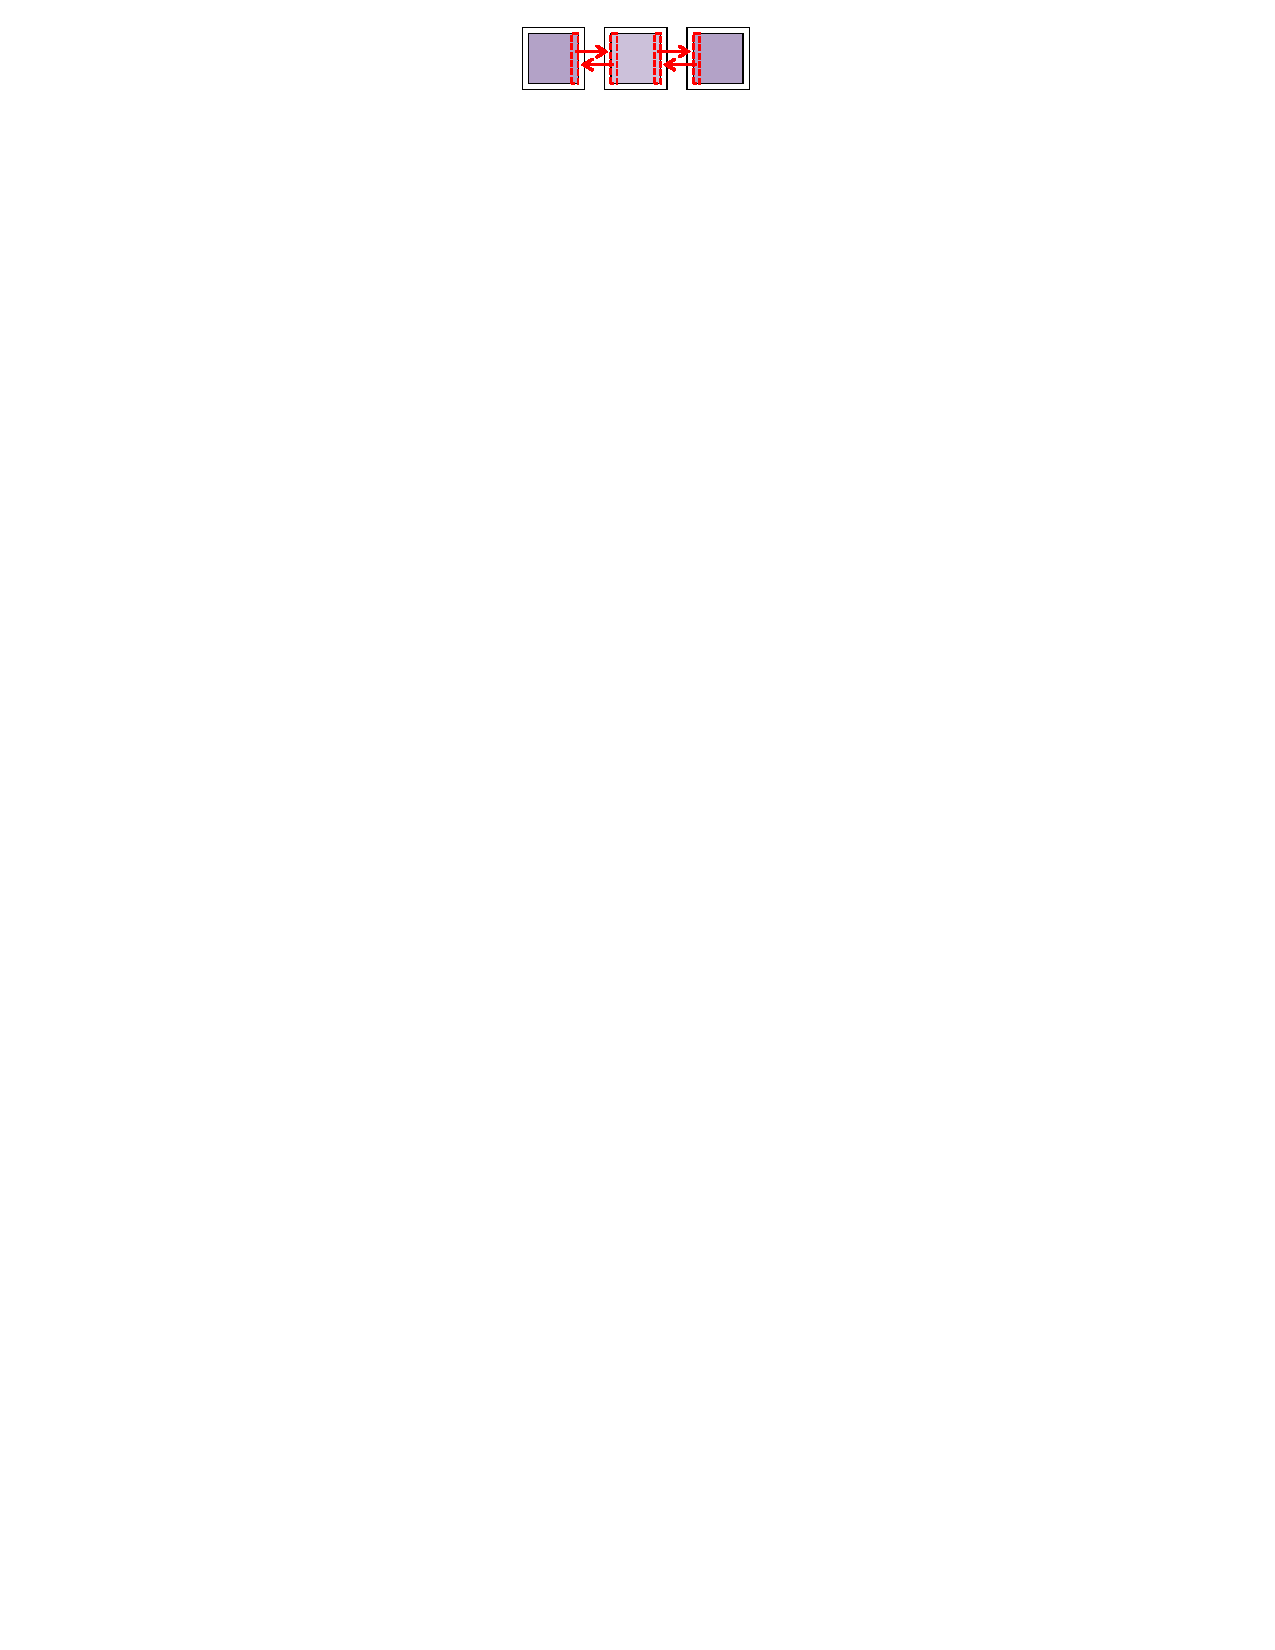
\includegraphics[trim=85mm 261mm 85mm 0mm, scale=0.8,clip]{figs/3cell-z.pdf}}  \\
%   \fbox{\includegraphics[trim=82mm 230mm 84mm 0mm, scale=0.8,clip]{figs/9cell-yz.pdf}}
%   \caption{3cell-y.pdf, 3cell-z.pdf, 9cell-yz.pdf}\label{fig:cell}
%   \end{center}
% \end{figure}


%-- fx100-pipo.pdf
%    \fbox{\includegraphics[trim=4mm 15mm 4mm 3mm, scale=0.9,clip]{figs/fx100-pipo.pdf}}

%himeno.pdf
%latency-16var.pdf
%layer.pdf

%register-CA-tmp.pdf
%register-RA-CA-tmp.pdf
%register-RA-tmp.pdf
%softstack.pdf
%translator-tmp.pdf


\section{Related Work}\label{sec:related}

%-- Coarray Imprementations
The University of Rice has implemented coarray features with their own extension 
called CAF2.0~\cite{Rice}.
It is a source-to-source compiler based on the ROSE compiler. GASNet is used as its 
communication layer.
Similarly to our RS and RA methods, they use the Cray pointer to pass the data 
allocated in C into Fortran.
%
Houston University developed UH-CAF onto the Open64-base OpenUH compiler~\cite{HU}. 
It supports coarray features defined in the Fortran 2008 standard. As the communication 
layer, GASNet and ARMCI can be used selectively.
%
OpenCoarrays is an open-source software project~\cite{OpenCo}. It is an library 
which can be used with GNU Fortran (gfortran) V5.1 or later. It supports coarray features
specified in Fortran 2008 and a part of Fortran 2018.  As the communication layer,
MPICH and GASNet can be used selectively.
%
In the vendors, Cray and Intel fully and Fujitsu partially support the coarray features
specified in Fortran 2008.

In the latest Fortran standard Fortran~2018, a subset of coarrays is called team.
It is similar to the executing images in the term of XMP, but does not affect
the parallel execution among images.

While non-blocking PUT communication is effective, non-blocking GET communication
is difficult to put into practical use because the acquired data is used immediately.
Cray has the directive extension for prefetching remote coarray corresponding to 
the GET communication.

Coarray C++ is a coarray implementation into C++. The coarray features are implemented
with the template library unlike XMP/C based on C language.



\section{Conclusion}\label{sec:concl}

本章では、XMPの文脈の中におけるcoarray featuresの位置付けを示し、
Omni XMP compilerの中での特徴的な実装を紹介した。

%-- 実装の特徴:library階層

評価では、同じローカルビューを記述するプログラミングモデルである
MPI message passingと比較し、性能の特徴を

%-- 実装の特徴: contiguity重視

実測を元にして処理系の性能を評価した。
Coarray featuresは

XMPの中でローカルビューを担うcoarray featuresは、性能

その価値と言えるローカルビュープログラミングの性能を評価した。



\section*{Acknowledgments}
                                   
The present research used the computational resources of HA-PACS provided by the 
Interdisciplinary Computational Science Program at the Center for 
Computational Sciences at the University of Tsukuba. 

Part of the results is obtained by using the K computer at the RIKEN Advanced 
Institute for Computational Science. %(Proposal number ra000002). 


\begin{thebibliography}{99}
\addcontentsline{toc}{chapter}{\bibname}

\bibitem{xmp} 
XcalableMP Language Specification, \url{http://xcalablemp.org/specification.html}

\bibitem{coarray} 
John Reid, JKR Associates, UK. Coarrays in the next Fortran Standard.
ISO/IEC JTC1/SC22/WG5 N1824, April 21, 2010.

\bibitem{coarray18} ISO/IEC TS 18508:2015, Information technology -- 
Additional Parallel Features in Fortran, Technical Specification, December 1, 2015.

\bibitem{omni} 
Omni Compiler Project. http://omni-compiler.org

\bibitem{pgas15} 
Hidetoshi Iwashita, Masahiro Nakao, Mitsuhisa Sato. 2015. Preliminary Implementation 
of Coarray Fortran Translator Based on Omni XcalableMP. PGAS2015, Proceedings of 9th 
International Conference on PGAS Programming Models, pp.70-75, Washington, D.C., USA.
September, 2015.

\bibitem{EPCC} EPCC Fortran Coarray micro-benchmark suite.\\
https://www.epcc.ed.ac.uk/research/computing/performance-characterisation-and-benchmarking/epcc-co-array-fortran-micro

\bibitem{himeno} 
Himeno Benchmark. \url{http://accc.riken.jp/en/supercom/himenobmt/}

\bibitem{Rice} 
John Mellor-Crummey, Laksono Adhianto, William N. Scherer III, and Guohua Jin. 
PGAS’09, 3rd Conference on Partitioned Global Address Space Programming Models. 
Ashburn, VA. October, 2009.

\bibitem{HU}
Deepak Eachempati, Hyoung Joon Jun, and Barbara Chapman. 
An Open-Source Compiler and Runtime Implementation for Coarray Fortran. 
PGAS’10, 4th Conference on Partitioned Global Address Space Programming Models, 
No.13. 2010.

\bibitem{OpenCo} 
Alessandro Fanfarillo, Tobias Burnus, Valeria Cardellini, Salvatore Filippone, 
Dan Nagle, and Damian Rouson. OpenCoarrays: Open-source Transport Layers 
Supporting Coarray Fortran Compilers, PGAS'14, Proc. of 8th International 
Conference on Partitioned Global Address Space Programming Models, No. 4. 2014.


% \bibitem{mpi} 
% MPI: A Message-Passing Interface Standard, \url{http://mpi-forum.org} 

% \bibitem{fj-mpi}
% Naoyuki Shida, Shinji Sumimoto, and Atsuya Uno. 
% MPI Library and Low-Level Communication on the K computer, 
% FUJITSU Scientific \& Technical Journal, Vol.48, No.3, pp.324–330. 2012. 

% \bibitem{asia18}
% Hidetoshi Iwashita, Masahiro Nakao, Hitoshi Murai and Mitsuhisa Sato. 
% A Source-to-Source Translation of Coarray Fortran with MPI for High Performance, 
% HPC Asia 2018, Proceedings of the International Conference on High Performance 
% Computing in Asia-Pasific Region, pp.86-97, Tokyo, Japan. January, 2018.

\end{thebibliography}


% OpenCoarrays. http://www.opencoarrays.org

% XcalableMP Specification Working Group. 2014. XcalableMP Language Specification 
% Version 1.2.1. http://www.xcalablemp.org/specification.html

% David Henty. 2012. A Parallel Benchmark Suite for Fortran Coarrays. In 
% Applications, Tools and Techniques on the Road to Exascale Computing, Advances 
% in Parallel Computing, Vol.22, pp.281-288.


% [12]Cristian Coarfa. 2007. Portable High Performance and Scalability of Global 
% Address Space Languages. Ph.D. Thesis, Rice University (Jan. 2007).

%[15]Shiyao Ge, Deepak Eachempati, Dounia Khaldi, and Barbara Chapman. 2015. 
%An Evaluation of Anticipated Extensions for Fortran Coarrays, PGAS’15, 9th 
%International Conference on Partitioned Global Address Space Programming Models, 
%P47-58, Washington, D.C. USA (Sep. 2015).


\end{document}



